\documentclass[a4paper]{paper}
\usepackage[utf8]{inputenc}
\usepackage[margin=2.5cm]{geometry}
\usepackage{enumitem}
\usepackage{float}
\usepackage[labelfont=bf,textfont=md]{caption}
\usepackage{graphicx}
\usepackage{xcolor}
\usepackage{minted}
\usepackage[square,numbers]{natbib}
\usepackage{hyperref}
\usepackage[all]{hypcap}
\usemintedstyle[common-lisp]{default}
\newmintinline[code]{text}{}
\bibliographystyle{plainnat}

\hypersetup{
  colorlinks,
  linkcolor={red!50!black},
  citecolor={blue!50!black},
  urlcolor={blue!80!black}
}

\newlist{step}{enumerate}{10}
\setlist[step]{label*=\arabic*.,leftmargin=2em}

\title{Using a Highly Dynamic Language for Development}
\subtitle{Advantages of and lessons learned from using Common Lisp in games}
\author{Nicolas Hafner}
\institution{Shirakumo Games}

\begin{document}
\twocolumn[\maketitle]

\begin{abstract}
  Games face an interesting challenge. They require rapid development, are highly interactive, and pose soft real-time performance constraints. While smaller games these days have also been developed in dynamic languages such as Python or Lua, traditionally engines are still written in static languages like C++ and C, with an additional scripting language on top to handle gameplay mechanics. Common Lisp offers an environment that's both dynamic and performant enough to allow for a full stack game development system that is highly favourable to fast iteration and modular design.
\end{abstract}
\begin{keywords}
  Common Lisp, game development, dynamic languages, object orientation
\end{keywords}

\def\abovecaptionskip{1pt}
\def\listingautorefname{Listing}
\def\figureautorefname{Figure}

\section{Introduction}
Video games pose an interesting engineering challenge. They are highly dynamic in their nature, as users can perform various, sometimes far-reaching changes to the program at any time, and yet they must remain responsive under soft real-time constraints. Additionally, the development of games itself is highly dynamic, as changes to the game require constant testing and refinement. Long pauses between making a change and being able to properly evaluate its effects can gravely discourage testing, which leads to a much worse product.

A typical approach to solve this set of constraints is to use multiple languages in combination. A rather low-level language like C++ or C to handle the ``core engine'', and an integrated scripting language like Lua to handle gameplay logic. However, this approach has multiple issues of its own: it can be hard to distinguish which parts should be a part of the core engine, and which should not. The scripting cannot integrate with everything the engine offers, as an explicit interface has to be designed that can deal with the scripting language's own data types and routines. For performance reasons a highly dynamic part may also need to be lowered down into the static language, making iteration much slower and harder to deal with.

Finally, the lack of runtime debugging means that any problems appearing in the core engine often lead to a crash of the entire program, which makes diagnosing and fixing the issue much harder. This difficulty often leads to defensive programming strategies, where errors are simply ignored or otherwise coerced, leading them to cause issues further down the line, complicating debugging of the final product even more.

In this paper we instead take a holistic approach, using Common Lisp for the full stack of both the core engine and the gameplay tools and mechanics. Common Lisp is a highly dynamic language, allowing runtime redefinition of functions, variables, and classes, even to the point of completely reloading or changing an underlying library or system while the program is being executed. Yet, despite this dynamism, Common Lisp is a compiled language that takes great care to support the writing of efficient code. Highly optimising compilers like SBCL allow you to write fast code without having to drop down into another language.

We explore some of the aspects of Common Lisp that make it particularly suited for games in detail, and also discuss some of the pitfalls we encountered and how to combat them.

\section{Related Works}
Please see our prior work on using Common Lisp for game development and real-time computer graphics\cite{hafner2018shader}\cite{hafner2019shader}. As this is otherwise primarily an overview of Common Lisp facilities and our experiences, we do not compare this paper to other work.

\section{Modularity Through Mixins}
The Common Lisp Object System (CLOS) has a couple of traits that remain rare in programming languages in use today, but make for excellent tools to support game development. Relevant to this section are serialised multiple inheritance and the standard generic function method combination. These features can be used to implement a system resembling ECS, though also offer a few advantages that make combination of behaviours more natural.

In CLOS methods are not attached to classes, but are instead parts of a generic function. Methods ``specialise'' on one or several of the required arguments of the function to a class. When the generic function is called, the system must first determine the set of ``applicable methods''. This set depends on the method combination used by the generic function. For brevity's sake, we will only look at the standard method combination here.

The standard method combination offers methods in four flavours: \code{primary}, \code{:before}, \code{:after}, and \code{:around}. These methods are grouped together, then filtered for applicable methods by checking whether the arguments passed to the generic function match their specialised classes, and finally sorted by \textit{how} specific the specialisations are to the arguments passed. With this completed set, the methods are invoked as illustrated in \autoref{fig:method combination}.

\begin{figure}[h]
  \centering
  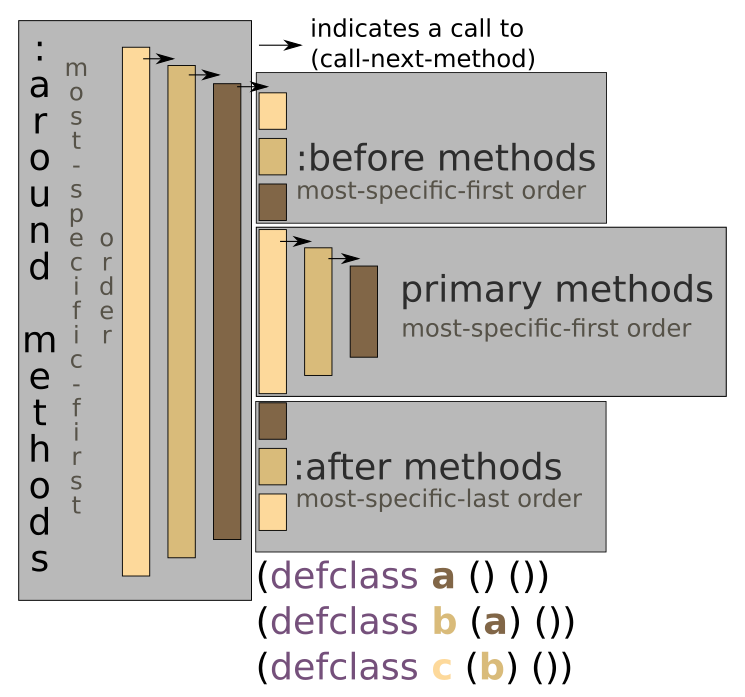
\includegraphics[width=0.45\textwidth]{method combination.png}
  \caption{The standard method combination behaviour illustrated}
  \label{fig:method combination}
\end{figure}

As a brief example, let us consider \autoref{lst:method definition}. Here we define a generic function of two arguments called \code{handle}, as well as three methods. All of the methods require the first argument to be a subclass of \code{tick}. Method 1 and 2 also require the second argument to be a subclass of \code{player}, and method 3 a subclass of \code{enemy}.

\begin{listing}[h]
\begin{minted}[fontsize=\scriptsize]{common-lisp}
(defgeneric handle (event object))

(defmethod handle         ((ev tick) (object player))) ; 1
(defmethod handle :before ((ev tick) (object player))) ; 2
(defmethod handle         ((ev tick) (object enemy)))  ; 3
\end{minted}
\caption{A brief example of method definition}
\label{lst:method definition}
\end{listing}

\hypertarget{first-call}{When \code{handle} is now called with a \code{tick} and a \code{player} instance, first the method 2 is executed, followed by the method 1. Method 3 is ignored, as it does not match the arguments.}

This method combination mechanism only really shines once we consider inheritance and especially multiple inheritance and the arising ``mixin classes''. Let us now define the classes we used for the previous listing. \autoref{lst:inheritance} shows five classes being defined, with \code{tick} being a subclass of \code{event}, and \code{player} and \code{enemy} being subclasses of \\\code{physics-object}.

\begin{listing}[H]
\begin{minted}[fontsize=\scriptsize]{common-lisp}
(defclass event () ())
(defclass tick (event) ())

(defclass physics-object () ())
(defclass player (physics-object) ())
(defclass enemy (physics-object) ())
\end{minted}
\caption{A brief example of method definition}
\label{lst:inheritance}
\end{listing}

We'll now also change the second method to specialise on the \code{physics-object} instead of \code{player}. For example, since both \code{player} and \code{enemy} are moving, we could be handling the collision resolution there. If we now perform the \hyperlink{first-call}{same call from before}, Methods 2 and 1 will still be invoked. However, unlike before, if we call the function with \code{tick} and \code{enemy}, now methods 2 and 3 will be invoked, instead of only method 3.

\begin{listing}[h]
\begin{minted}[fontsize=\scriptsize]{common-lisp}
(defmethod handle :before ((ev tick) (object physics-object)))
\end{minted}
\caption{The updated second method definition}
\label{lst:updated method}
\end{listing}

In other OOP paradigms a similar behaviour can usually be achieved by calling the superclass' method with \code{super}, but notice here that the behaviour of method 2 does not require changing anything about the other methods or subclasses. It thus remains wholly encapsulated in its own behaviour.

So far so good. Now imagine that we decide enemies, should emit a light so that they're always visible. To implement this, we're going to define a new class, \code{emitter}, and define the light flicker behaviour in a new \code{handle} method as shown in \autoref{lst:emitter}.

\begin{listing}[h]
\begin{minted}[fontsize=\scriptsize]{common-lisp}
(defclass emitter () ())

(defmethod handle :before ((ev tick) (object emitter)))
\end{minted}
\caption{The new class and method to handle light flickering}
\label{lst:emitter}
\end{listing}

To make the enemy adopt this new behaviour, all we need to do is add \code{emitter} to the \code{enemy} class' superclass list. Thanks to the method combination, calls to \code{handle} will now include the \code{emitter}'s method, and we have achieved the combination of the two behaviours.

\begin{listing}[H]
\begin{minted}[fontsize=\scriptsize]{common-lisp}
(defclass enemy (physics-object emitter) ())
\end{minted}
\caption{The updated enemy class definition}
\label{lst:new-enemy}
\end{listing}

The order of the superclasses here is important. Classes that appear earlier in the list have ``precedence'' and are thus considered to be ``more specific'' when determining the set of applicable methods. By having \code{emitter} appear after \code{physics-object}, we ensure that the \code{emitter}'s \code{:before} method runs \textit{after} that of \code{physics-object}, ensuring the collisions have already resolved properly once we consider the lighting update.

Not having the \code{emitter} be a subclass of \\\code{physics-object} ensures that we can also use it as a superclass for other things such as completely static lanterns that have no business having any interactivity.

As an example from our actual code base, as of writing, the \code{player} class has 8 direct superclasses whose behaviours are combined together with the \code{player}'s own. This combination of behaviours allows encapsulating different parts and re-using them in many cases. Keep in mind, too, that all of these classes and methods can be redefined at runtime to change, add, and remove behaviours from an object while the game is still running.

We've also developed a system to tie shaders into the CLOS inheritance model, allowing us to attach GPU rendering behaviour to classes, and combine it in a similar fashion\cite{hafner2019shader}.

One issue that crops up when segregating behaviours into such small compartments is that you might not have enough control over the combination of them. The standard method combination offers no fine-grained control to exclude or reorder methods for a specific specialisation of an argument. One could devise their own method combination strategy to allow this kind of specialised behaviour, however we are not convinced that this would not lead to an ultimately even more confusing design.

While the standard method combination and mixins offer a great deal of flexibility out of the box, great care must still be taken when designing the overall class hierarchy and function protocol. Otherwise behaviours will not combine cleanly and lead to strange bugs, or might not combine properly at all.

\section{Conditions, Handlers, and Restarts}
Debugging is of course an important aspect of programming, but this is even more so the case when the system can be redefined and changed during runtime. Fortunately, Common Lisp offers an incredibly capable system to deal with runtime bugs. This system comes in three parts, only one of which is commonly found in other languages.

The first part is what's called ``conditions'', or Exceptions in other languages. Conditions are ``signalled'' (thrown) and can then be ``handled'' (caught) by a piece of code lower down in the stack. When handled, the stack unwinds to the point of the handler, and the matching handler function is invoked to resolve the issue. For our purposes here, Common Lisp offers two types of conditions: warnings and errors. When a warning is signalled that is not handled further up the stack, it simply vanishes and execution continues from the signalling point unimpeded. If an error remains unhandled, a dynamic debugger is invoked instead and the signalling thread is paused. From there one of the unique features comes to shine.

Restarts are on first look similar to conditions and handlers. When a restart is established through \code{restart-case}, it sets an unwind point for a particularly named restart with a function to be called when that restart is triggered. Restarts themselves can be triggered via a function called \code{invoke-restart}, which can also pass along arguments for the restart function. The idea with restarts is to provide one or more ways for execution to continue or recover safely from an error. When the debugger is invoked from an unhandled error, it now has access to a list of active restarts on the stack, and can invoke one of them dynamically as the user sees fit.

This means that unlike traditional languages where an error causes a stack trace and then tries to continue or simply crashes, in Common Lisp execution is halted, waiting for you to analyse and potentially fix the bug. Once you're confident you know what to do or have solved the issue, you can pick from one of several ways to continue the execution from the error. This leaves the program running at all times and means you don't need to worry about long recompilation times or setup times to reproduce the error, you can immediately continue where you left off.

The debugger also allows you to evaluate expressions at runtime while in a particular stack frame, allowing access to local variables in the process. Since the Common Lisp runtime includes the full compiler suite at all times, these expressions can be arbitrary Lisp code, allowing for far more invasive exploration of the bug and changes to the environment than easily possible with traditional out-of-process debuggers.

The final piece is the existence of \code{handler-bind}. This is a type of handler for conditions, but unlike the regular handlers that cause the stack to unwind, these handlers are invoked \textit{on top of the stack} of where the condition was signalled. As such they have full access to the dynamic environment at error point. In fact, this is also how the top level debugger is invoked. However, with \code{handler-bind} you can automate the error resolution and avoid requiring user input.

A system with well-designed recovery points through restarts can then be set up to automatically recover from most errors in a way much more refined than traditional Exceptions, as there is an inversion of control.

\begin{listing}[H]
\begin{minted}[fontsize=\scriptsize]{common-lisp}
(defmethod render ((scene scene))
  (for ((object in scene))
    (restart-case
        (render object)
      (continue ())))

(defmethod render ((main main))
  (handler-bind ((error (lambda (condition)
                          (invoke-restart 'continue))))
    (render (scene main))))
\end{minted}
\caption{Simplified code illustrating the control inversion of restarts}
\label{lst:restarts}
\end{listing}

In \autoref{lst:restarts} we show two simple methods, the first to render a \code{scene}, which simply iterates over each object in the scene and establishes a \code{continue} restart around the call to \code{render} the object. When this restart is invoked, the stack unwinds to within the \code{for} and then simply continues with the next object.

If we now call \code{render} on a \code{scene} directly and an error occurs, the debugger gets invoked as usual. But this time, we can invoke the \code{continue} restart from the debugger to skip rendering the object. We could also define a ``retry'' restart to simply retry rendering the object as well, if we wanted to.

However, importantly, for the \code{main} \code{render}\\ method, this restart is automatically invoked, ensuring that any potential crashes at runtime of the game are gracefully ignored. This handler could also be defined elsewhere even higher up the stack, or only invoke the restart under special conditions. This works as the \code{lambda} of the \code{handler-bind} is invoked at the point of error on top of the stack, where the \code{continue} restart is visible.

Restarts and handlers are fantastic tools to create a more error friendly environment and to recover from unfavourable situations. Combined with the dynamic debugger and runtime compilation environment, these tools make debugging problems and evolving a system over time a lot easier.

\section{Optimisation}
A frequent problem with highly dynamic language is optimisation, as the dynamic nature of the language prohibits making assumptions at compile time, forcing repeated runtime dispatching. The focus on safety will also insert bounds checks and similar assertions into the code, which can have a big impact on runtime in the hot loop.

To help with these issues, Common Lisp includes several tools in the form of sorts of ``compiler promises''. You can use a declaration to promise to the compiler that a variable's value assumes a certain type. The compiler can then use this promise to perform inference and eliminate runtime dispatching. SBCL is often times good enough at automatically inferring the types to eliminate much of runtime dispatch on its own, but for highly optimised functions, declaring the types manually can be very beneficial still.

Additionally, Common Lisp offers several compiler tuning declarations. For instance, increasing the \code{speed} switch to its maximum will tell the compiler to try and optimise the code as much as it can. SBCL will then also emit warnings about cases where it doesn't have sufficient information to eliminate dispatch, or where it must allocate on the heap. Using this extra information the programmer can then refactor the code or add additional promises to ensure the compiler can generate efficient code.

Another switch is the \code{safety} switch, which when set to its minimum will tell the compiler to avoid inserting safety checks such as runtime type checks, bounds checks, or other features that typically help catch bugs. Naturally this is a dangerous option, as the generated code now becomes as unsafe as C or assembly code, and misuse of functions declared with this option can lead to memory corruptions.

You can also declare the type of a function, to ensure that the compiler can infer return values and arguments across function boundaries. SBCL's block compilation feature, when activated, also allows it to reason across function boundaries within the same compilation unit on its own.

Finally you can also declare functions to be \code{inline}, allowing the compiler to inline the definitions at call sites. This comes with the usual advantage of aiding inference and removing call overhead, but does hamper dynamism, as a change to an inlined function now requires recompiling call sites as well.

When focusing on the SBCL implementation, there are several other optimisations that can be done. SBCL offers full access to its code optimisation facilities and even its assembler routines. With enough effort, code can be optimised on the assembly level, and one could even emit special assembly instructions where needed. Some libraries already make use of these systems to speed up computations, but we have not touched them much ourselves due to a lack of time so far. We do however make use of the \code{disassemble} function to check the generated assembly of functions, as another aid in optimisation. We also make use of the integrated statistical profiler to observe the runtime of the game and determine choke points.

These techniques mostly focus on type dispatch within a function, with special focus on arithmetic functions. Dispatch for generic functions cannot be eliminated like this, and especially generic functions with a lot of methods attached or complicated method signatures can become a significant choke point.

This can be largely combated with traditional techniques of simplifying method signatures, splitting up generic functions, or rewriting them into statically dispatching functions that can be inlined to take advantage of type inference. We are also investigating an alternate dispatch technique outlined by Robert Strandh\cite{strandh2014fast} that should significantly improve generic function dispatch time, potentially even outperforming traditional vtable based approaches as used in C++ or Java.

While all these opportunities mean that fast code can be written in SBCL, the default is still on the side of safety over performance, something we consider an ultimately good thing. Fully optimising code on the level of C, C++, or assembly requires significant, but not insurmountable work.

\section{Garbage Collection}
Being such a highly dynamic language, it's unavoidable that a garbage collector be involved. This can be problematic for games where a GC cycle can easily eclipse the time budget of a single frame. There already exists a breadth of literature on the topic of GC types, GC tuning, etc. out there so we will not go into a debate on the nature of GC or its drawbacks and advantages here. Instead we will focus on the specific issues we have encountered and what we've done to mitigate them.

The GC we use is SBCL's default GC, a generational, compacting, single-threaded stop-the-world collector. We do hope that SBCL will receive a better GC such as the Memory Pool System\cite{brooksby2002memory} at some point, but for now we've been focusing on minimising garbage production in our code to avoid frequent and extensive GCs.

Garbage can be minimised in a number of ways, the most general being object pooling, or in other words manual garbage collection. By allocating\\known needed objects ahead of time and simply recycling them, we can avoid generating a lot of intermittent garbage. Common Lisp gives us some very useful tools here that make this process a lot easier.

For instance, we can ask the compiler to allocate a number of objects on the stack by using a declaration (\code{(declare (dynamic-extent x))}). However, this only works if the compiler can know ahead of time what size the object is, meaning only fixed size arrays and known structs can be stack allocated. Furthermore, stack space is much more limited, so bigger allocations still have to happen on the heap.

For cases where the object is a class instance, simply too big for the stack, or has to escape the stack sometimes, we can still easily cache the instance locally by using \code{load-time-value}.\\\code{load-time-value} is a special operator that causes the form it wraps to be executed when the code is first loaded into the system, and then puts the result of that executed form in the place in the code the \code{load-time-value} was at. This effectively creates an anonymous global variable where the object is stored, which is then put in place of the original \code{load-time-value}.

This trick is very useful when we know the code path is only ever accessed from one thread at a time. Multi-threaded schemes would need to employ more complex methods.

Another point where \code{load-time-value} becomes very useful is when objects are said to be immutable, and their construction arguments are known at compile time. In this case, we can define a ``compiler macro'' which is a macro that is executed to replace a call to a particular function. This compiler macro can then analyse the arguments to the function at compile-time and choose to substitute the call with a \code{load-time-value} form if all arguments can be determined statically. This then avoids the construction and allocation of the object, or even the entire computation of the function at runtime in a, to the user, completely transparent fashion.

In Alloy, our UI toolkit, we use this trick extensively to avoid the allocation of colour values, sizes, and dimensional units.

Even with all of these tricks, it remains very hard to completely eliminate allocations, as other parts such as boxing of values or generation of bignums can cause allocations in spots where it isn't immediately obvious. So far we have managed to keep the game running smoothly enough by offloading big GC cycles to load screens and transitions, but it is clear that bigger games do need additional work put into them to optimise them for garbage management.

\section{Conclusion}
The expressiveness of the Common Lisp Object System allows for rapid changes in game object behaviour, as well as the creation of reusable pieces of behaviour that can often be seamlessly combined together. With extensions to the Meta Object Protocol, this can even be extended to graphics rendering routines and shaders.

The presence of the entire compiler environment at runtime allows the developer to change any part of the game while it is running. This is especially feasible thanks to the presence of the restarts and interactive debugger, which allow the game to recover from a bug without having to crash and restart the entire system.

While these features offer great amounts of flexibility, there is a performance cost. Many of these performance penalties can be avoided or circumvented with careful planning and design, but often by sacrificing some of the dynamism. These optimisations also come at a greater development cost.

We believe that, since these optimisations can be performed gradually over time and because no optimisation opportunities are fundamentally excluded, Common Lisp still makes for a great candidate language for game development.

While there are many more intricacies to the Common Lisp ecosystem, we hope that this paper gives a brief insight into some of the advantages and challenges present when working in a full stack Common Lisp environment.

\section{Acknowledgements}
We would like to thank the very handsome and attractive people that helped proofread this draft ;)

\bibliography{paper}
\end{document}


%%% Local Variables:
%%% mode: latex
%%% TeX-command-extra-options: "-shell-escape"
%%% TeX-master: t
%%% TeX-engine: luatex
%%% End:
